\documentclass[12pt]{article}
\usepackage{ctex}
\usepackage{graphicx}
\usepackage{indentfirst}
\usepackage{amsmath}
\usepackage{float}
\usepackage{amssymb}
\usepackage{bm}
\title{第十三周作业报告}
\author{佐藤拓未 20300186002}
\date{}

\begin{document}
	
	
	
	
	\maketitle
	
	
	\begin{center}
		\textbf{第一问}
	\end{center}
\noindent 实现Dirichlet-Neumann方法求解二维的Poisson方程, 并观察收敛速度与差分网格步长$h$的关系.\\
\quad \\
\textbf{解:} 考虑给定一个二维的Poisson方程, 
\begin{align*}
	\begin{cases}
		-\Delta u = f,\quad & x \in \Omega = (0,1)\times(0,1)\\
		u = 0, &x\in {\rm \partial}\Omega 
	\end{cases}
\end{align*}
\noindent 为了进一步考虑数值与真解在D-N方法下的误差, 可以给定特别的非齐次项$f=-2[x_1(x_1-1)+x_2(x_2-1)]$, 可知其真解为$u(x_1,x_2)=x_1x_2(x_1-1)(x_2-1)$. 在进一步给定划分区域: $\Gamma = \{x_1=\frac{1}{2},x_2\in(0,1)\}$, $\Omega_1=\{ x_1 \in(0,\frac{1}{2}), x_2 \in(0,1)       \}$, $\Omega_2 = \{x_1 \in(\frac{1}{2},1),x_2\in(0,1)\}$.\\
\quad \\
下面考虑Dirichlet-Neumann方法: 首先给定$u_2^0$在交界面$\Gamma$的初始猜想值$u_2^0=g^0$.\\
为了叙述方便, 统一定义括号外右下标$(x_1)_i$代表着$x_1$轴的第$i$个分量, 即$(x_1)_i=i\cdot h_{x_1}$; $(u_1^k)_{i,j}$对应于$((x_1)_i,(x_2)_j)$.\\
\textbf{Step 1:} 在$\Omega_1$上求解Dirichlet边值问题:
\begin{align*}
	-\Delta u_1^k =f&,\quad \quad  in \quad \Omega_1\\
	u_1^k=0&,\quad \quad  on \quad   {\rm \partial}\Omega_1 \cap {\rm \partial}\Omega\\
	u_1^k=g^{k-1}&, \quad \quad on \quad \Gamma 
\end{align*}
\noindent 因此在$\Omega_1$上求解问题时, 只需要对$(u^k_1)_{N-1,j}$所对应的列向量分量$f_{N-1,j}$进行修改(其中下标$(N-1,j)$对应于$((x_1)_{N-1},(x_2)_{j})$), 即$f_{N-1,j}\rightarrow f_{N-1,j}+\frac{1}{h_{x_1}^2}\cdot (g^{k-1})_{N,j}$.\\
另一方面, 为了求解在$\Omega_1=\{ x_1 \in(0,\frac{1}{2}), x_2 \in(0,1)       \}$上的五点差分线性方程组, 我们需要五点差分矩阵$A$是一个方阵, 从而我们可以得出$h_{x_1}=\frac{h_{x_2}}{2}$.
\noindent \textbf{Step 2:} 在$\Omega_2$上求解Neumann边值问题:
\begin{align*}
	-\Delta u_2^k=f&,\quad \quad in \quad \Omega_2\\
	u_2^k=0&,\quad \quad on \quad {\rm \partial}\Omega_2 \cap {\rm \partial}\Omega\\
	\frac{{\rm \partial }u_2^k}{{\rm \partial }n_2}=-\frac{{\rm \partial }u_1^k}{{\rm \partial }n_1}&,\quad \quad on \quad \Gamma
\end{align*}
其中注意到在交界面$\Gamma$上有$\frac{{\rm \partial }u_2^k}{{\rm \partial }n_2}=-\frac{{\rm \partial }u_1^k}{{\rm \partial }n_1}$, 即关于$\Gamma$的法向方向导数. 又$\Gamma=\{x_1=\frac{1}{2},x_2\in(0,1)\}$, 可知方向导数$\frac{{\rm \partial }u_2^k}{{\rm \partial }n_2}=\frac{{\rm \partial }u_2^k}{{\rm \partial }x_1},\frac{{\rm \partial }u_1^k}{{\rm \partial }n_1}=\frac{{\rm \partial }u_1^k}{{\rm \partial }x_1}$, 再由数值上有
\begin{align*}
	-\frac{{\rm \partial }u_1^k}{{\rm \partial }x_1}(\frac{1}{2},(x_2)_j)&\approx \frac{(u^{k}_{1})_{N-1,j}-(u^k_{1})_{N,j}}{h_{x_1}},\quad \\
	-\frac{{\rm \partial }u_2^k}{{\rm \partial }x_1}(\frac{1}{2},(x_2)_j)&\approx \frac{(u^{k}_{2})_{N+1,j}-(u^k_{2})_{N,j}}{h_{x_1}},\\
	(u^k_2)_{N,j}&=\frac{(u^k_2)_{N+1,j}+(u^k_2)_{N-1,j}}{2}
\end{align*}
\noindent 上面两式中$(u^k_1)_{N,j},(u^k_2)_{N,j}$代表了在第$k$步迭代中, 分别在$\Omega_1,\Omega_2$上考虑在$\Gamma$上的值; $(u_1^k)_{N-1,j}$说明在数值上近似$\Omega_1$的外法向量时用到了前一步的值; $(u_2^k)_{N+1,j}$说明在数值上近似$\Omega_2$的外法向量时用到了后一步的值. 最终, 在$\Omega_2$上求解五点差分格式的线性方程组, 我们需要同时修改矩阵$A$与列向量$f$: $(A)_{(i-1)(N-1)+1,(i-1)(N-1)+1}\rightarrow(A)_{(i-1)(N-1)+1,(i-1)(N-1)+1}-\frac{1}{2h_x^2}$, 以及$f_{(i-1)(N-1)+1,1}\rightarrow f_{(i-1)(N-1)+1,1}+\frac{1}{2h_x^2}\cdot(u^k_1)_{N-1,i}$.\\
\textbf{Step 3:} 更新$g^k$:$$g^k=\theta u^k_2\vert _\Gamma +(1-\theta)g^{k-1}$$
\noindent 由于DN方法分别在$\Omega_1$与$\Omega_2$上求解五点差分格式, 从而最终得到的数值解内点$(u)_{i,j}$对应于$(2N-1)\times(N-1)$的网格.\\
\quad \\
下面考虑数值解与真解的误差与网格步长$h_{x_1}=\frac{h_{x_2}}{2}$的关系\\
\noindent \underline{当$\theta=0.5$, 迭代步数$k=5$时的收敛速度}: 考虑$h_{x_2}=2^{-n},h_{x_1}=\frac{h_{x_2}}{2}$, 下图为$n=2,\cdots,6$时的每点误差.
\begin{figure}[H]
	\centering
	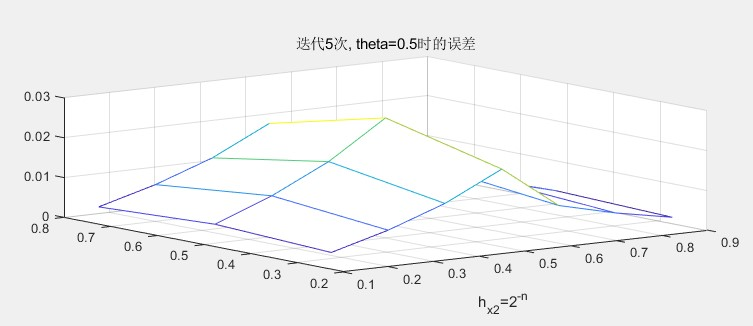
\includegraphics[width=1\textwidth]{1}
	\caption{当$n=2$时的误差}
\end{figure}
\begin{figure}[H]
	\centering
	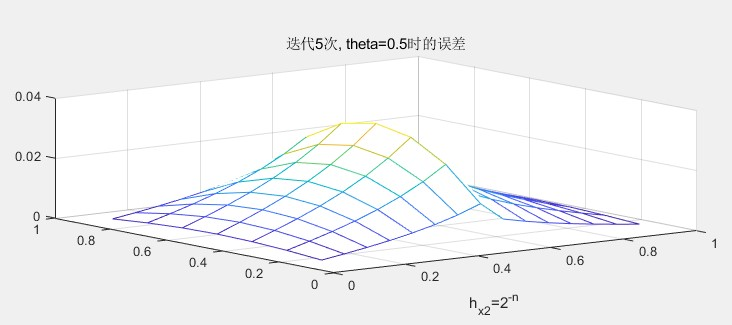
\includegraphics[width=1\textwidth]{2}
	\caption{当$n=3$时的误差}
\end{figure}
\begin{figure}[H]
	\centering
	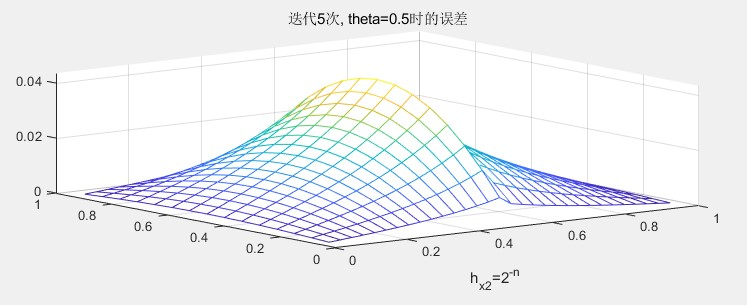
\includegraphics[width=0.85\textwidth]{3}
	\caption{当$n=4$时的误差}
\end{figure}
\begin{figure}[H]
	\centering
	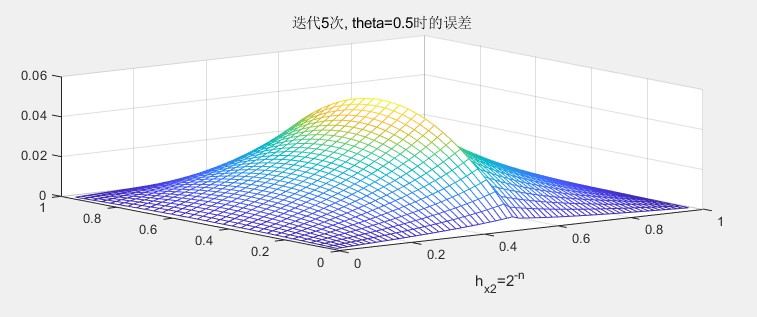
\includegraphics[width=0.85\textwidth]{4}
	\caption{当$n=5$时的误差}
\end{figure}
\begin{figure}[H]
	\centering
	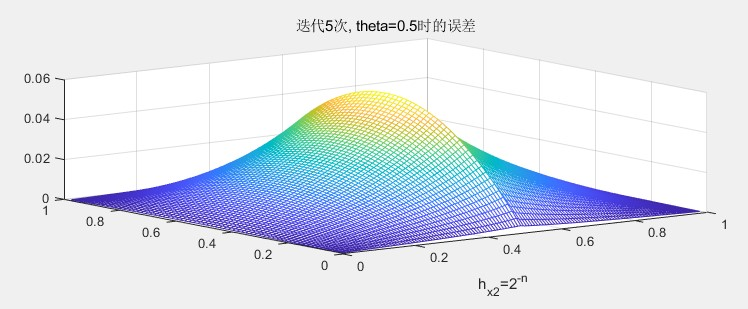
\includegraphics[width=0.85\textwidth]{5}
	\caption{当$n=6$时的误差}
\end{figure}
\begin{figure}[H]
	\centering
	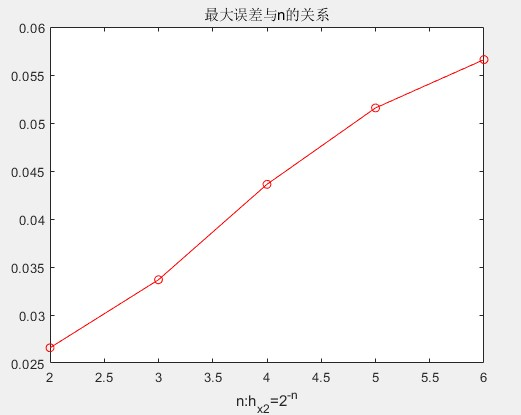
\includegraphics[width=0.85\textwidth]{6}
	\caption{最大误差与$n$的关系, 迭代5次}
\end{figure}
\noindent 可以发现当$n$增大时, 更细的网格下的最大误差反而增大了, 误差增大的可能原因如下: 1) 在$\Omega_2$上考虑Neumann边界条件时, 考虑的是分别用向后与向前差商近似两个外法向量, 从而引入了误差; 2) 迭代次数不够多.\\
而当迭代次数够大时, 可以发现随着$n$增大时, 最大误差是下降的, 且是一阶收敛的, 见图7.\\
除上所述, 可以发现$\forall n = 2,\cdots,6$, 最大误差总是在$\Gamma$上取到, 这会令我们联想到取不同的权重$\theta$是否会影响到误差?
\begin{figure}[H]
	\centering
	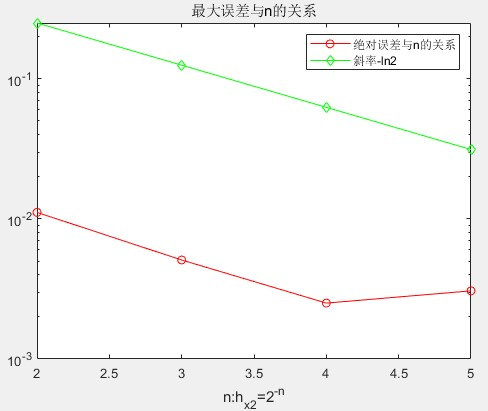
\includegraphics[width=0.85\textwidth]{7}
	\caption{最大误差与$n$的关系, 迭代70次}
\end{figure}
\quad \\
\noindent \underline{当$\theta=0.7,k=5$时}: 可以发现情形稍有改善, 但仍然在$\Gamma$上取到最大误差
\begin{figure}[H]
	\centering
	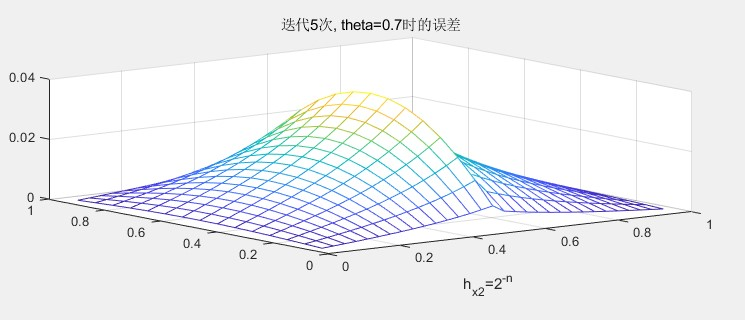
\includegraphics[width=0.85\textwidth]{8}
	\caption{当$n=6,k=5$时的误差}
\end{figure}
\begin{figure}[H]
	\centering
	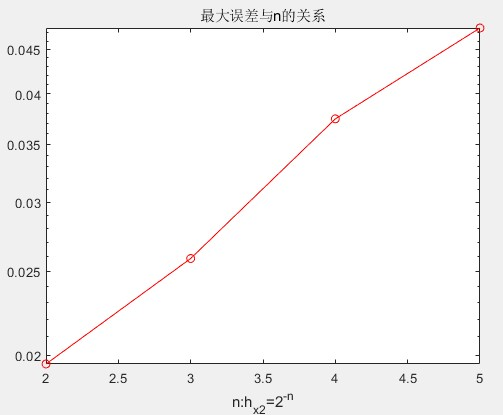
\includegraphics[width=0.7\textwidth]{9}
	\caption{最大误差与$n$的关系, 迭代5次,$\theta=0.7$}
\end{figure}
\begin{figure}[H]
	\centering
	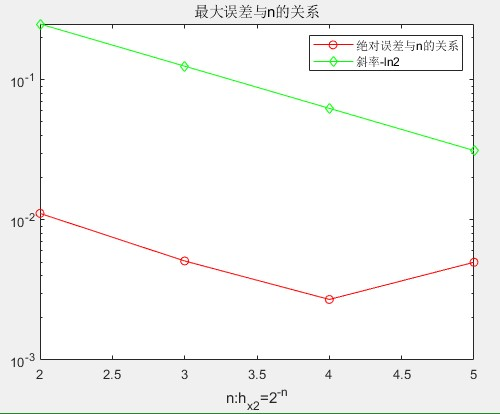
\includegraphics[width=0.7\textwidth]{10}
	\caption{最大误差与$n$的关系, 迭代40次,$\theta=0.7$}
\end{figure}
\noindent 当迭代次数$k$较小时, 随着$n$的增大, 网格精度反而升高变差了, 如图9所示. 而当迭代次数增加时, 当$n$增大时, 细网格的收敛速度会变得越来越显著, 呈现最大误差的一阶收敛性, 如图10所示.\\
\quad \\
\noindent 在此题中, 我选择分别在$\Omega_1$与$\Omega_2$上求解Dirichlet与Neumann初边值问题, 从而使得横纵坐标网格的步长$h$并不一样. 从结果来看, 这种DN方法所求解得出的数值解在迭代次数较少时, 与真解的误差并不会随着$n$的增大而减小; 但是当迭代次数较大时, 随着$n$的增大, 越细的网格的收敛速度越发显著. 而这样的网格也具有以下缺点; 1) 并不能在迭代次数较少时获得较好的收敛速度 2) 在考虑$\Omega_2$上的Neumann问题时, 考虑的两个外法向量均是由向前或者向后差商所逼近, 因此容易引起扰动, 从而导致在$\Gamma$处会取到较大的误差.
\end{document}